\documentclass[]{article}
\usepackage{lmodern}
\usepackage{amssymb,amsmath}
\usepackage{ifxetex,ifluatex}
\usepackage{fixltx2e} % provides \textsubscript
\ifnum 0\ifxetex 1\fi\ifluatex 1\fi=0 % if pdftex
  \usepackage[T1]{fontenc}
  \usepackage[utf8]{inputenc}
\else % if luatex or xelatex
  \ifxetex
    \usepackage{mathspec}
  \else
    \usepackage{fontspec}
  \fi
  \defaultfontfeatures{Ligatures=TeX,Scale=MatchLowercase}
\fi
% use upquote if available, for straight quotes in verbatim environments
\IfFileExists{upquote.sty}{\usepackage{upquote}}{}
% use microtype if available
\IfFileExists{microtype.sty}{%
\usepackage{microtype}
\UseMicrotypeSet[protrusion]{basicmath} % disable protrusion for tt fonts
}{}
\usepackage[margin=1in]{geometry}
\usepackage{hyperref}
\hypersetup{unicode=true,
            pdfborder={0 0 0},
            breaklinks=true}
\urlstyle{same}  % don't use monospace font for urls
\usepackage{graphicx,grffile}
\makeatletter
\def\maxwidth{\ifdim\Gin@nat@width>\linewidth\linewidth\else\Gin@nat@width\fi}
\def\maxheight{\ifdim\Gin@nat@height>\textheight\textheight\else\Gin@nat@height\fi}
\makeatother
% Scale images if necessary, so that they will not overflow the page
% margins by default, and it is still possible to overwrite the defaults
% using explicit options in \includegraphics[width, height, ...]{}
\setkeys{Gin}{width=\maxwidth,height=\maxheight,keepaspectratio}
\IfFileExists{parskip.sty}{%
\usepackage{parskip}
}{% else
\setlength{\parindent}{0pt}
\setlength{\parskip}{6pt plus 2pt minus 1pt}
}
\setlength{\emergencystretch}{3em}  % prevent overfull lines
\providecommand{\tightlist}{%
  \setlength{\itemsep}{0pt}\setlength{\parskip}{0pt}}
\setcounter{secnumdepth}{0}
% Redefines (sub)paragraphs to behave more like sections
\ifx\paragraph\undefined\else
\let\oldparagraph\paragraph
\renewcommand{\paragraph}[1]{\oldparagraph{#1}\mbox{}}
\fi
\ifx\subparagraph\undefined\else
\let\oldsubparagraph\subparagraph
\renewcommand{\subparagraph}[1]{\oldsubparagraph{#1}\mbox{}}
\fi

%%% Use protect on footnotes to avoid problems with footnotes in titles
\let\rmarkdownfootnote\footnote%
\def\footnote{\protect\rmarkdownfootnote}

%%% Change title format to be more compact
\usepackage{titling}

% Create subtitle command for use in maketitle
\providecommand{\subtitle}[1]{
  \posttitle{
    \begin{center}\large#1\end{center}
    }
}

\setlength{\droptitle}{-2em}

  \title{}
    \pretitle{\vspace{\droptitle}}
  \posttitle{}
    \author{}
    \preauthor{}\postauthor{}
    \date{}
    \predate{}\postdate{}
  

\begin{document}

\hypertarget{probabilidad-los-fundamentos}{%
\section{Probabilidad: los
fundamentos}\label{probabilidad-los-fundamentos}}

\hypertarget{el-rol-de-la-probabilidad-en-estaduxedstica}{%
\subsection{El rol de la probabilidad en
Estadística}\label{el-rol-de-la-probabilidad-en-estaduxedstica}}

Para hacer inferencias se requiere de la probabilidad porque se trabaja
con situaciones inciertas, que no se conocen y que son difíciles de
prever. Por eso se comienza aquí haciendo la distinción entre las
preguntas que pueden responderse con certeza y las que no. De las
primeras, son ejemplos: ¿cuándo será el próximo eclipse de sol? ¿Cómo
varía el diámetro de la pupila luego del consumo de alcohol? Sobre estas
preguntas tenemos, o bien un conocimiento profundo sobre el movimiento
de los astros, o bien una gran cantidad de observaciones, que nos
permiten dar una respuesta certera.

Por el contrario, si preguntamos ¿cuál es el efecto sobre la
personalidad, de haber tenido figuras parentales autoritarias en la
niñez? ¿Qué determina que algunos alumnos tengan éxito en la escuela y
otros no? ¿Cómo afecta la estabilidad económica a la intención de voto?,
solo podemos ofrecer respuestas parciales, tentativas, aproximadas. Se
trata de hechos que dependen de muchos factores a los que no conocemos
en su totalidad, por lo que el resultado es variable: algunas personas
criadas en ambientes autoritarios desarrollan una personalidad
autoritaria, otras no. En algunos alumnos, el hecho que sus padres
tengan estudios elevados los ayuda a tener éxito en la escuela, pero
también hay hijos de personas muy educadas que fracasan en la escuela.
La estabilidad económica que favorecería una reelección, puede estar
acompañada de mucha pobreza, o de corrupción; también eventos
inesperados antes de las elecciones pueden cambiar decisiones a último
momento. Hay razones más allá de nuestro alcance que inciden en la
personalidad o en el resultado de la escuela, o la intención de voto. En
estas situaciones, cuando no tenemos toda la información que hace falta
para predecir el resultado, recurriremos a la probabilidad.

Ingresaremos al tema desde situaciones muy sencillas, desde el muy usado
ejemplo de arrojar una moneda. Pero detengámonos un momento en él: si
tuviéramos toda la información necesaria para predecir la trayectoria de
la moneda en el aire (distancia desde donde se arroja, fuerza que se le
aplica, el lugar de la moneda donde se aplica esa fuerza, eventuales
corrientes de aire que puedan incidir en el desplazamiento de la moneda,
etc.), podríamos predecir con certeza el resultado. Esa información no
está disponible, el lado del que caiga la moneda está determinado por
una multiplicidad de factores, por esa razón no podemos anticipar el
resultado de la tirada. A esa ignorancia la resumimos diciendo que el
resultado de la tirada de la moneda ``depende del azar'' y llamamos al
experimento de tirar una moneda ``experimento aleatorio''.

Es un paso muy largo ir desde este ejemplo a decir que el modo en que se
desarrolle la personalidad de alguien que ha sido criado en una familia
autoritaria depende del azar o que la distribución de votos en las
próximas elecciones depende del azar. Sabemos que esos resultados no
dependen del azar, dependen de muchos factores que ignoramos, por eso
usaremos probabilidades en las disciplinas que tratan con sujetos
humanos, por la imposibilidad de predecir con certeza los resultados.
Podremos decir que un alumno cuyos padres valoran la educación tiene una
probabilidad mayor de tener éxito en la escuela, pero no podremos
asegurar que lo tendrá. Es razonable creer que si un gobierno logró
estabilidad económica, tendrá más posibilidades de ser reelegido, pero
no hay certeza sobre que lo será. Los tratamientos más exitosos
encuentran casos en los que no logran resultados, por lo que su
efectividad no puede garantizarse completamente, hay una componente
impredecible en la evolución de la patología.

La probabilidad trata con la incertidumbre, con lo que hay entre la
certeza en que algo ocurrirá y la certeza en que no ocurrirá.

Los eventos que no son azarosos no tienen que ver con probabilidades: no
asignamos probabilidad a un eclipse porque hay conocimiento suficiente
como para saber cuándo ocurrirá; pero sí se asigna probabilidad a una
tormenta, porque no se conocen simultáneamente todos los factores que la
determinan. Se asignan probabilidades a hechos de cuya ocurrencia no se
tiene certeza. Con la probabilidad se cuantifica (se le asigna un
número) a la expectativa sobre el fenómeno. Intuitivamente, cuando
decimos que algo tiene ``mucha probabilidad de suceder'' es porque
estamos bastante seguros que sucederá. Esta es la posición conocida como
``azar epistemológico'', que considera azarosos o aleatorios a los
eventos cuya ocurrencia no puede anticiparse con certeza. Desde esta
posición, que sea azaroso o no, depende el conocimiento que se tenga
sobre los determinantes del evento.

La cuantificación de la probabilidad implica que ésta se expresa con un
número que está comprendido entre cero y uno. Que un evento tenga
probabilidad cero significa que es imposible que suceda. Si un evento
tiene probabilidad igual a uno, se llama ``evento seguro'', y quiere
decir que hay certeza en que sucederá.

\hypertarget{formas-para-asignar-probabilidades}{%
\subsection{Formas para asignar
probabilidades}\label{formas-para-asignar-probabilidades}}

\hypertarget{asignaciuxf3n-a-priori}{%
\subsubsection{Asignación a priori}\label{asignaciuxf3n-a-priori}}

Podemos partir de esa idea intuitiva de probabilidad, ligada a procesos
cuya ocurrencia no nos es conocida con certeza. Para evocar esta idea,
el ejemplo que más a menudo se cita es el del lanzamiento de una moneda,
¿cuál es la probabilidad de obtener ``cara'' al arrojar una moneda? Si
la respuesta es \(1/2\) (o 0,50 ó 50 y 50), debe tenerse en cuenta que
eso solo será cierto si la moneda está equilibrada, es decir si tiene
iguales chances de salir de un lado que del otro. Si esto es cierto,
efectivamente la probabilidad de obtener cara es \(1/2\) (ó 0,50). Con
idéntica condición, la probabilidad de obtener un 5 al arrojar un dado
es \(1/6\) (ó 0,17). Esta asignación de probabilidad a los resultados de
un experimento es previa a su realización, no es necesario tirar
realmente la moneda: es suficiente con que tengamos razones para
\emph{suponer} que está equilibrada, para poder afirmar que la
probabilidad de cara es \(1/2\). Diremos en este caso que asignamos la
probabilidad \emph{a priori}, es decir, antes de hacer el experimento.

De mismo modo sucede si el evento que nos interesa en un poco más
complejo. Por ejemplo: ¿Cuál es la probabilidad de obtener un número
mayor a cuatro si se tira un dado? Debido a que hay dos números mayores
a cuatro (5 y 6), el evento tiene dos casos a su favor y hay seis
resultados posibles, por lo que la probabilidad será: \(2/6\) (ó
\(1/3\), si se simplifica la fracción).

La expresión formal de esta asignación de probabilidades es.

\[P(A)=\frac{\#A}{\#\Omega}\]

En la que \(\#A\) (que se lee ``numeral de A'') indica el número de
maneras enque puede suceder el evento A, y \(\#\Omega\) (numeral de
omega) es el número total de resultados que se pueden obtener al
realizar el experimento. \(\Omega\) es el conjunto de resultados
posibles, es llamado \emph{espacio muestral}. En el caso del ejemplo, el
experimento es el de tirar el dado y buscar un número mayor que cuatro,
\(\#A\) es 2 porque son las formas en que puede obtenerse un número
mayor que cuatro, y \(\#\Omega\) es 6, que es el número total de
resultados posibles al tirar un dado.

Con este mismo razonamiento, la probabilidad de obtener un número par es
\(3/6\) (\(1/2\) después de simplificar), porque hay tres números pares
(2, 4 y 6) en un dado.

Vamos a un caso más complejo: tiremos ahora dos dados y tomemos en
cuenta la suma de los dos puntajes, a esa suma la llamaremos \(S\). El
mínimo número que puede resultar es dos (que ambos dados salgan uno) y
el máximo es doce (ambos seis), entonces hay once resultados posibles de
esta variable (que son: \(S = 2\), \(S = 3\), \(S = 4\), \(S = 5\),
\(S = 6\), \(S = 7\), \(S = 8\), \(S = 9\), \(S = 10\), \(S = 11\) y
\(S = 12\)), algunos de los cuales pueden suceder de varias formas.
Estos resultados posibles y sus formas de obtención se ven de manera
esquemática a continuación:

\begin{table}

\caption{\label{tab:unnamed-chunk-7}Resultados posibles de la suma de los puntajes de dos dados.}
\centering
\begin{tabular}[t]{lccccccc}
\toprule
\multicolumn{2}{c}{ } & \multicolumn{6}{c}{Primer dado} \\
\cmidrule(l{3pt}r{3pt}){3-8}
 &  & **1** & **2** & **3** & **4** & **5** & **6**\\
\midrule
\rowcolor{gray!6}   & **1** & 2 & 3 & 4 & 5 & 6 & 7\\
\cmidrule{2-8}
 & **2** & 3 & 4 & 5 & 6 & 7 & 8\\
\cmidrule{2-8}
\rowcolor{gray!6}   & **3** & 4 & 5 & 6 & 7 & 8 & 9\\
\cmidrule{2-8}
 & **4** & 5 & 6 & 7 & 8 & 9 & 10\\
\cmidrule{2-8}
\rowcolor{gray!6}   & **5** & 6 & 7 & 8 & 9 & 10 & 11\\
\cmidrule{2-8}
\multirow[t]{-6}{*}{\raggedright\arraybackslash Segundo dado} & **6** & 7 & 8 & 9 & 10 & 11 & 12\\
\bottomrule
\end{tabular}
\end{table}

Si bien los resultados posibles son 11, las formas en que estos pueden
darse son 36; cada una de esas formas es un evento. El evento primer
dado 5 y segundo dado 2 es diferente del evento primer dado 2 y segundo
dado 5, aunque ambos conducen al mismo resultado de la suma: \(S=7\).
Más precisamente, si indicamos los eventos con pares ordenados, los
eventos \((1,6)\); \((6,1)\); \((2,5)\); \((5,2)\); \((3,4)\); \((4,3)\)
son diferentes pero todos corresponden a \(S=7\).

Son entonces 36 los resultados posibles del experimento, por lo que
\(\#\Omega\) = 36. Ahora podemos calcular probabilidades para diferentes
resultados.

¿Cuál es la probabilidad que la suma sea 12?, lo que puede expresarse
como: ¿cuál es \(P(S=12)\)? Como esta suma solo puede lograrse si ambos
dados salen 6, hay una sola manera en que se produzca el evento que nos
interesa (suma doce), por lo que el \(\#A\) es 1 y la probabilidad es
entonces \(1/36\).

\begin{quote}
\(\#A = 1, P(S = 12)=1/36\)
\end{quote}

\begin{table}[H]
\centering
\begin{tabular}{lccccccc}
\toprule
\multicolumn{2}{c}{ } & \multicolumn{6}{c}{Primer dado} \\
\cmidrule(l{3pt}r{3pt}){3-8}
 &  & **1** & **2** & **3** & **4** & **5** & **6**\\
\midrule
\rowcolor{gray!6}   & **1** & 2 & 3 & 4 & 5 & 6 & 7\\
\cmidrule{2-8}
 & **2** & 3 & 4 & 5 & 6 & 7 & 8\\
\cmidrule{2-8}
\rowcolor{gray!6}   & **3** & 4 & 5 & 6 & 7 & 8 & 9\\
\cmidrule{2-8}
 & **4** & 5 & 6 & 7 & 8 & 9 & 10\\
\cmidrule{2-8}
\rowcolor{gray!6}   & **5** & 6 & 7 & 8 & 9 & 10 & 11\\
\cmidrule{2-8}
\multirow[t]{-6}{*}{\raggedright\arraybackslash Segundo dado} & **6** & 7 & 8 & 9 & 10 & 11 & **\_12\_**\\
\bottomrule
\end{tabular}
\end{table}

En cambio, si la pregunta es por la probabilidad de obtener un tres, hay
más de una manera de llegar a ese resultado (que \(S = 3\)). La suma 3
puede resultar de \(2+1\) ó de \(1+2\), es decir que, o bien el primer
dado sale 2 y el segundo 1 ó bien el primero sale 1 y el segundo 2. Hay
así dos formas posibles para el evento \(S = 3\), y \(\#A\) es 2, por lo
que la probabilidad es \(P(S = 3) = 2/36\).

\begin{quote}
\(\#A = 2, P(S = 3)=2/36\)
\end{quote}

\begin{table}[H]
\centering
\begin{tabular}{lccccccc}
\toprule
\multicolumn{2}{c}{ } & \multicolumn{6}{c}{Primer dado} \\
\cmidrule(l{3pt}r{3pt}){3-8}
 &  & **1** & **2** & **3** & **4** & **5** & **6**\\
\midrule
\rowcolor{gray!6}   & **1** & 2 & **\_3\_** & 4 & 5 & 6 & 7\\
\cmidrule{2-8}
 & **2** & **\_3\_** & 4 & 5 & 6 & 7 & 8\\
\cmidrule{2-8}
\rowcolor{gray!6}   & **3** & 4 & 5 & 6 & 7 & 8 & 9\\
\cmidrule{2-8}
 & **4** & 5 & 6 & 7 & 8 & 9 & 10\\
\cmidrule{2-8}
\rowcolor{gray!6}   & **5** & 6 & 7 & 8 & 9 & 10 & 11\\
\cmidrule{2-8}
\multirow[t]{-6}{*}{\raggedright\arraybackslash Segundo dado} & **6** & 7 & 8 & 9 & 10 & 11 & 12\\
\bottomrule
\end{tabular}
\end{table}

Otro ejemplo, sea \(P(S=7)\). La suma de siete puede obtenerse de muchas
formas: \(1+6\), \(2+5\), \(3+4\), \(4+3\), \(5+2\) ó \(6+1\). Hay seis
combinaciones que conducen a \(S=7\), en consecuencia, la probabilidad
es \(6/36\).

\begin{quote}
\(\#A = 6, P(S = 7)=6/36\)
\end{quote}

\begin{table}[H]
\centering
\begin{tabular}{lccccccc}
\toprule
\multicolumn{2}{c}{ } & \multicolumn{6}{c}{Primer dado} \\
\cmidrule(l{3pt}r{3pt}){3-8}
 &  & **1** & **2** & **3** & **4** & **5** & **6**\\
\midrule
\rowcolor{gray!6}   & **1** & 2 & 3 & 4 & 5 & 6 & **\_7\_**\\
\cmidrule{2-8}
 & **2** & 3 & 4 & 5 & 6 & **\_7\_** & 8\\
\cmidrule{2-8}
\rowcolor{gray!6}   & **3** & 4 & 5 & 6 & **\_7\_** & 8 & 9\\
\cmidrule{2-8}
 & **4** & 5 & 6 & **\_7\_** & 8 & 9 & 10\\
\cmidrule{2-8}
\rowcolor{gray!6}   & **5** & 6 & **\_7\_** & 8 & 9 & 10 & 11\\
\cmidrule{2-8}
\multirow[t]{-6}{*}{\raggedright\arraybackslash Segundo dado} & **6** & **\_7\_** & 8 & 9 & 10 & 11 & 12\\
\bottomrule
\end{tabular}
\end{table}

\hypertarget{asignaciuxf3n-a-posteriori}{%
\subsubsection{Asignación a
posteriori}\label{asignaciuxf3n-a-posteriori}}

Consideremos ahora una situación más cercana a la experiencia:
supongamos que de un curso se selecciona un alumno al azar ¿Cuál es la
probabilidad que sea mujer? Aquí el supuesto de equilibrio no es válido
a priori, en gran medida depende de la carrera de que se trata, las hay
con muchas mujeres y con pocas. Por lo tanto no podemos suponer que es
igualmente probable que resulte un varón o una mujer y no podemos
asignar probabilidad \(1/2\) a cada resultado. Aunque el experimento
tenga dos resultados posibles, éstos no son igualmente probables.

En otro ejemplo, si al alumno aleatoriamente seleccionado (por ejemplo,
el que ocupa el lugar 40 en la lista de inscriptos) se le pregunta por
el tipo de colegio del que egresó, con los resultados posibles:
``público'', ``privado laico'', ``privado religioso'', el resultado que
se obtenga también depende del azar, porque así fue elegido el alumno,
la respuesta será una u otra según cuál sea el alumno elegido y esto
depende del azar. Sin embargo, no podemos asignar una probabilidad igual
a cada resultado, no es lícito decir que sea \(1/3\), ya que puede haber
más estudiantes que provengan de colegios públicos que de privados y, en
consecuencia, que sea más probable encontrar alumnos provenientes de
esos colegios que de los otros. En este caso no podemos asignar de
antemano probabilidades a los diferentes resultados, porque no tenemos
suficientes razones para suponer \emph{la forma en que se distribuyen}
las probabilidades. Si supiéramos que hay el doble de alumnos que vienen
de colegios públicos, podríamos decir que el alumno elegido al azar
tiene el doble de probabilidad de provenir de un colegio público que de
otro tipo.

Encontramos así una relación entre la frecuencia y la probabilidad: si
conocemos la distribución de frecuencias, tenemos razones para usarlas
para asignar probabilidades a los resultados del experimento. Así, si
una muestra de alumnos ofrece la siguiente distribución de frecuencias
para el tipo de colegio del que provienen.

\begin{table}

\caption{\label{tab:unnamed-chunk-11}Distribución de frecuencias del tipo de colegio del que provienen alumnos que ingresan a la universidad}
\centering
\begin{tabular}[t]{lcc}
\toprule
 & f & f'\\
\midrule
\rowcolor{gray!6}  Público & 200 & 0,66\\
Privado laico & 20 & 0,07\\
\rowcolor{gray!6}  Privado religioso & 80 & 0,27\\
Total & 300 & 1,00\\
\bottomrule
\multicolumn{3}{l}{\textit{Fuente: } datos ficticios para ejemplificación.}\\
\end{tabular}
\end{table}

Estamos autorizados a decir que la probabilidad que el alumno elegido al
azar provenga de un colegio público es 0,67, que es su frecuencia
relativa. Esto será válido en la medida que el número de casos sea
elevado; no es posible transformar una frecuencia relativa en
probabilidad si tenemos muy pocas observaciones. Más adelante volveremos
sobre esta importante limitación.

Cuando atribuimos probabilidades de este modo se trata de probabilidades
\emph{a posteriori}, es decir con posterioridad a haber hecho la
experiencia, luego de la observación de los resultados reales obtenidos.
También se llama a estas probabilidades \emph{empíricas}, para destacar
que provienen de la experiencia.

¿Cuál es el significado del 1.00 que corresponde al total? Sin dudas,
como frecuencia significa el 100\% de los casos, pero como probabilidad
indica que el conjunto completo de alternativas (público, privado laico,
privado religioso) tiene probabilidad 1.00; o bien que es un
\emph{evento seguro}. La expresión coloquial para este valor es que
cuando se selecciona un alumno al azar, éste debe provenir de alguno de
los tres tipos de colegio indicados, entonces el valor uno responde a la
pregunta ``¿cuál es la probabilidad de encontrar un alumno que provenga
de un colegio que sea público, privado laico o privado religioso?'', la
respuesta es que es seguro que de alguno de esos tipos de colegio
provendrá el alumno, porque no hay otras alternativas, es decir que las
categorías son exhaustivas, como debe ser. En este caso,

\[\mathrm{\Omega} = \{ publico,\ privado\ laico,\ privado\ religioso\}\]

Como vimos más arriba, el evento seguro es el que tiene probabilidad 1,
por lo que la expresión formal de este enunciado es:

\(P(\Omega) = 1\)

Donde \(\Omega\) indica el conjunto de todos los resultados posibles de
un experimento aleatorio, o el conjunto de todas las categorías de un
variable, al que hemos llamado \emph{espacio muestral}.

\hypertarget{la-relaciuxf3n-entre-asignaciuxf3n-a-priori-y-a-posteriori}{%
\subsubsection{La relación entre asignación a priori y a
posteriori}\label{la-relaciuxf3n-entre-asignaciuxf3n-a-priori-y-a-posteriori}}

Volvamos al experimento simple de arrojar la moneda: si ésta se
encuentra equilibrada será entonces correcto asignar probabilidad
\(1/2\) (ó 0,50) a cada lado, lo que indica que esperamos que \emph{a la
larga} la moneda caiga la mitad de las veces cara y la mitad cruz.
Destaquemos la expresión ``a la larga'', que quiere decir ``si se arroja
muchas veces''. Hagamos el experimento realmente, busque usted una
moneda y arrójela, digamos 10 veces. Yo lo hice y obtuve la siguiente
secuencia de resultados: CXXXCCCXXC.

Elijamos nuestro lado favorito, que sea ``cara'' (C) y calculemos la
frecuencia relativa de ese lado en cada tirada, presentamos los
resultados resumidamente en la tabla . Cuando solo la he tirado una vez
y como el primer resultado fue C, la frecuencia es 1 (una cara de un
total de un resultado). A la segunda tirada, que es X, se obtiene
\(1/2\) (una cara de dos tiradas). A la tercera, que otra vez sale X, la
frecuencia de cara es \(1/3\) (una cara de tres tiradas) y así sigue:

\begin{table}

\caption{\label{tab:unnamed-chunk-12}Frecuencias relativas correspondientes a una secuencia de diez lanzamientos de una moneda.}
\centering
\begin{tabular}[t]{lcccc}
\toprule
Tirada & Cantidad de tiradas & Resultado & Cantidad de caras acumuladas & Frecuencia relativa del evento "cara"\\
\midrule
\rowcolor{gray!6}  Primera & 1 & C & 1 & 1/1 = 1,00\\
Segunda & 2 & X & 1 & 1/2 = 0,50\\
\rowcolor{gray!6}  Tercera & 3 & X & 1 & 1/3 = 0,33\\
Cuarta & 4 & X & 1 & 1/4 = 0,25\\
\rowcolor{gray!6}  Quinta & 5 & C & 2 & 2/5 = 0,40\\
\addlinespace
Sexta & 6 & C & 3 & 3/6 = 0,50\\
\rowcolor{gray!6}  Séptima & 7 & C & 4 & 4/7 = 0,57\\
Octava & 8 & X & 4 & 4/8 = 0,50\\
\rowcolor{gray!6}  Novena & 9 & X & 4 & 4/9 = 0,44\\
Décima & 10 & C & 5 & 5/10 = 0,50\\
\bottomrule
\end{tabular}
\end{table}

En la distribución vemos que la frecuencia relativa de C toma valores
alrededor de 0,50; al principio más lejos y luego ``se va acercando'' a
ese número cuando hemos hecho más tiradas. La representación gráfica de
este proceso es la siguiente:

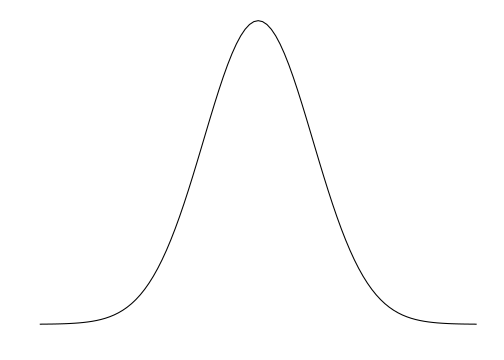
\includegraphics{08-capitulo7_files/figure-latex/unnamed-chunk-13-1.pdf}

Donde hemos agregado una línea que muestra el valor 0,50 que es el que
habíamos calculado antes de hacer el experimento. Se aprecia que la
sucesión de frecuencias relativas es tal que éstas se van acercando a la
probabilidad predicha. Si la moneda se hubiese tirado una cantidad mayor
de veces (cien veces, por ejemplo), el gráfico tendría una forma como la
siguiente:

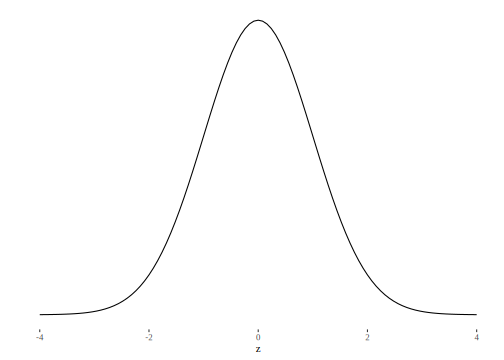
\includegraphics{08-capitulo7_files/figure-latex/unnamed-chunk-14-1.pdf}

Resulta entonces que, si se cumple que la moneda está equilibrada,
entonces las frecuencias relativas de un resultado se irán acercando a
la probabilidad asignada. Dicho de otra manera, la probabilidad a
posteriori converge a la probabilidad a priori. Mucha atención a esto:
solo en el caso que el supuesto inicial se cumpla, es decir que la
moneda se comporte como esperamos (cayendo parejo de un lado y del
otro).

Si por el contrario, la moneda estuviese desequilibrada -y que fuera más
frecuente el lado X que el lado C-, podríamos obtener, en 500 tiradas,
por ejemplo, 350 veces X y la probabilidad a posteriori será entonces
\(P(C) = 350/500 = 0,70\) y no 0,50 como sería si estuviera equilibrada.
En ese caso el supuesto inicial de moneda equilibrada se muestra falso,
decimos que ``el modelo no se sostiene'', en un momento veremos con más
detalle el significado de esta expresión.

\hypertarget{operando-con-probabilidades}{%
\subsection{Operando con
probabilidades}\label{operando-con-probabilidades}}

Cualquiera sea el modo a través del que se hayan asignado probabilidades
a eventos, las probabilidades cumplen con ciertas propiedades generales,
que trataremos a continuación y que permiten hacer operaciones con
ellas.

En primer lugar, y con carácter de axiomas, las siguientes
características son condición para que un número \(P(A)\) pueda ser
considerado una probabilidad:

\begin{itemize}
\item
  La probabilidad es un número comprendido entre cero y uno:
  \(0 \leq P(A) \leq 1\)
\item
  La probabilidad del conjunto completo de resultados posibles (del
  espacio muestral) es uno: \(P(\Omega) = 1\)
\item
  La probabilidad de la unión de dos eventos que se excluyen mutuamente
  es la suma de las probabilidades de cada uno de ellos:
  \(P(A \cup B) = P(A) + P(B)\)
\end{itemize}

La definición frecuencial (a posteriori), así como todos los modelos de
asignación de probabilidad a priori que mencionamos cumplen con estas
condiciones.

\hypertarget{con-probabilidades-frecuenciales}{%
\subsubsection{Con probabilidades
frecuenciales}\label{con-probabilidades-frecuenciales}}

Sea una distribución conjunta de dos variables con asignación de
probabilidades frecuenciales, es decir empíricas. Se trata de la
relación entre la ciudad donde se vive y la intención de voto. Las
categorías de la ciudad son: Córdoba, Rosario y Mendoza. Los partidos
políticos son cuatro y los llamaremos Q, R, S y T. Supongamos que las
siguientes son las frecuencias observadas luego de recoger los datos:

\begin{table}

\caption{\label{tab:unnamed-chunk-15}Distribución del partido al que declara que va a votar y la ciudad de residencia.}
\centering
\begin{tabular}[t]{lccccc}
\toprule
\multicolumn{1}{c}{Ciudad} & \multicolumn{4}{c}{Partido al que dice que votará} & \multicolumn{1}{c}{Total} \\
\cmidrule(l{3pt}r{3pt}){1-1} \cmidrule(l{3pt}r{3pt}){2-5} \cmidrule(l{3pt}r{3pt}){6-6}
 & Q & R & S & T & \\
\midrule
\rowcolor{gray!6}  Córdoba & 200 & 300 & 100 & 50 & 650\\
Rosario & 100 & 150 & 60 & 70 & 380\\
\rowcolor{gray!6}  Mendoza & 50 & 150 & 100 & 200 & 500\\
Total & 350 & 600 & 260 & 320 & 1530\\
\bottomrule
\end{tabular}
\end{table}

Calculemos algunas probabilidades a partir de las frecuencias relativas.

\hypertarget{probabilidades-marginales}{%
\paragraph{Probabilidades marginales}\label{probabilidades-marginales}}

Cuando se consideran las categorías de una variable sin tener en cuenta
a la otra, usamos las frecuencias de los márgenes de la tabla, esas son
las llamadas \textbf{frecuencias marginales}. La probabilidad que una
persona elegida al azar viva en Córdoba (sin importar a qué partido
piense votar) es \(650/1530\). De manera equivalente, la probabilidad de
encontrar por azar a alguien que piense votar al partido \(S\)
(cualquiera sea su ciudad) es \(260/1530\). Las escribimos simplemente
\(P(Córdoba)\) y \(P(S)\) respectivamente. En las tablas singuientes
están destacadas las frecuencias que participan en el cálculo de estas
probabilidades.

\begin{table}

\caption{\label{tab:unnamed-chunk-16}Distribución del partido al que declara que va a votar y la ciudad de residencia. Esquema para el cálculo de la probabilidad marginal $P(Córdoba)$.}
\centering
\begin{tabular}[t]{lccccc}
\toprule
\multicolumn{1}{c}{Ciudad} & \multicolumn{4}{c}{Partido al que dice que votará} & \multicolumn{1}{c}{Total} \\
\cmidrule(l{3pt}r{3pt}){1-1} \cmidrule(l{3pt}r{3pt}){2-5} \cmidrule(l{3pt}r{3pt}){6-6}
 & Q & R & S & T & \\
\midrule
\rowcolor{gray!6}  Córdoba & 200 & 300 & 100 & 50 & **650**\\
Rosario & 100 & 150 & 60 & 70 & 380\\
\rowcolor{gray!6}  Mendoza & 50 & 150 & 100 & 200 & 500\\
Total & 350 & 600 & 260 & 320 & **1530**\\
\bottomrule
\end{tabular}
\end{table}

\begin{table}

\caption{\label{tab:unnamed-chunk-17}Distribución del partido al que declara que va a votar y la ciudad de residencia. Esquema para el cálculo de la probabilidad marginal $P(S)$.}
\centering
\begin{tabular}[t]{lccccc}
\toprule
\multicolumn{1}{c}{Ciudad} & \multicolumn{4}{c}{Partido al que dice que votará} & \multicolumn{1}{c}{Total} \\
\cmidrule(l{3pt}r{3pt}){1-1} \cmidrule(l{3pt}r{3pt}){2-5} \cmidrule(l{3pt}r{3pt}){6-6}
 & Q & R & S & T & \\
\midrule
\rowcolor{gray!6}  Córdoba & 200 & 300 & 100 & 50 & 650\\
Rosario & 100 & 150 & 60 & 70 & 380\\
\rowcolor{gray!6}  Mendoza & 50 & 150 & 100 & 200 & 500\\
Total & 350 & 600 & **260** & 320 & **1530**\\
\bottomrule
\end{tabular}
\end{table}

\hypertarget{probabilidades-conjuntas-o-de-la-intersecciuxf3n-de-eventos}{%
\paragraph{Probabilidades conjuntas o de la intersección de
eventos}\label{probabilidades-conjuntas-o-de-la-intersecciuxf3n-de-eventos}}

Las usamos para hallar la probabilidad de ocurrencia simultánea de una
categoría de cada variable. Por ejemplo ¿Cuál es la probabilidad de
encontrar por azar a alguien que viva en Rosario años \textbf{y} que
piense votar al partido R? La cantidad de individuos que cumplen
\textbf{simultáneamente} las dos condiciones es de 150, por lo que la
probabilidad se calcula como \(150/1530\). Hemos destacado la conjunción
``y'', junto al ``simultáneamente'' porque en este caso se piden dos
condiciones juntas. Por eso estas son llamadas \textbf{probabilidades
conjuntas}.

En teoría de conjuntos, corresponden a la intersección de dos conjuntos,
que se indica con el signo \(\cap\), por lo que el evento ``vivir en
Rosario'' y al mismo tiempo ``decir que se va a votar a R'', se escribe
``\(Rosario \cap R\)''.

Esa intersección puede verse gráficamente en el cruce de la fila con la
columna correspondiente.

\begin{table}

\caption{\label{tab:unnamed-chunk-18}Distribución del partido al que declara que va a votar y la ciudad de residencia. Esquema para el cálculo de la probabilidad conjunta $P(Rosario y R)$.}
\centering
\begin{tabular}[t]{lccccc}
\toprule
\multicolumn{1}{c}{Ciudad} & \multicolumn{4}{c}{Partido al que dice que votará} & \multicolumn{1}{c}{Total} \\
\cmidrule(l{3pt}r{3pt}){1-1} \cmidrule(l{3pt}r{3pt}){2-5} \cmidrule(l{3pt}r{3pt}){6-6}
 & Q & R & S & T & \\
\midrule
\rowcolor{gray!6}  Córdoba & 200 & 300 & 100 & 50 & 650\\
Rosario & 100 & **150** & 60 & 70 & 380\\
\rowcolor{gray!6}  Mendoza & 50 & 150 & 100 & 200 & 500\\
Total & 350 & 600 & 260 & 320 & **1530**\\
\bottomrule
\end{tabular}
\end{table}

¿Qué sucede si aplicamos esta operación a dos eventos que corresponden a
dos categorías de la misma variable?, por ejemplo, ¿cuál es la
probabilidad de encontrar a alguien que diga que votará a Q y a R? Esos
eventos no pueden suceder juntos porque son incompatibles: solo uno de
los dos puede suceder. La intersección entre ellos es imposible, por lo
que la probabilidad es cero. Es el mismo caso de buscar a alguien que
viva en Córdoba y también en Mendoza, es claro que no hay intersección
entre estos conjuntos; dicho de otra forma, la intersección es el
conjunto vacío. A estos eventos que no pueden suceder simultáneamente,
los llamaremos mutuamente excluyentes. Como recordamos, esa es la
condición que deben cumplir las categorías de cualquier variable.

Si dos eventos son mutuamente excluyentes entonces, su probabilidad
conjunta es cero. En lenguaje de conjuntos:

\[si\ A \cap B = \varnothing\ entonces\ P(A \cap B) = 0\]

\hypertarget{probabilidad-de-la-uniuxf3n-de-eventos-mutuamente-excluyentes}{%
\paragraph{Probabilidad de la unión de eventos mutuamente
excluyentes}\label{probabilidad-de-la-uniuxf3n-de-eventos-mutuamente-excluyentes}}

Estas probabilidades sirven para analizar la ocurrencia de uno u otro de
dos eventos, cuando éstos no pueden suceder simultáneamente. Por
ejemplo: ¿qué probabilidad hay de encontrar a alguien que piense votar a
Q \textbf{o} a R? Esto quiere decir ``una cosa o la otra'', se trata de
una disyunción, es decir, la unión de los dos eventos. En el lenguaje de
la teoría de conjuntos la unión de dos conjuntos se indica con el
símbolo \(\cup\), por lo que decir ``A o B'' equivale a decir
``\(A\cup B\)''.

El total de quienes cumplen con la condición de votar a Q o a R (sin
tener en cuenta la ciudad) es de \(950 (350 + 600)\), por lo que la
probabilidad es de \(950/1530\).

\begin{table}

\caption{\label{tab:unnamed-chunk-19}Distribución del partido al que declara que va a votar y la ciudad de residencia. Esquema para el cálculo de la probabilidad $P(Q o R)$ (eventos disjuntos).}
\centering
\begin{tabular}[t]{lccccc}
\toprule
\multicolumn{1}{c}{Ciudad} & \multicolumn{4}{c}{Partido al que dice que votará} & \multicolumn{1}{c}{Total} \\
\cmidrule(l{3pt}r{3pt}){1-1} \cmidrule(l{3pt}r{3pt}){2-5} \cmidrule(l{3pt}r{3pt}){6-6}
 & Q & R & S & T & \\
\midrule
\rowcolor{gray!6}  Córdoba & 200 & 300 & 100 & 50 & 650\\
Rosario & 100 & 150 & 60 & 70 & 380\\
\rowcolor{gray!6}  Mendoza & 50 & 150 & 100 & 200 & 500\\
Total & **350** & **600** & 260 & 320 & **1530**\\
\bottomrule
\end{tabular}
\end{table}

De modo equivalente, la probabilidad de seleccionar al azar a alguien
que viva en Córdoba o en Rosario es de \(1030/1530\), donde hemos sumado
las dos primeras categorías (Córdoba y Rosario).

\begin{table}

\caption{\label{tab:unnamed-chunk-20}Distribución del partido al que declara que va a votar y la ciudad de residencia. Esquema para el cálculo de la probabilidad $P(Córdoba o Rosario)$ (eventos disjuntos).}
\centering
\begin{tabular}[t]{lccccc}
\toprule
\multicolumn{1}{c}{Ciudad} & \multicolumn{4}{c}{Partido al que dice que votará} & \multicolumn{1}{c}{Total} \\
\cmidrule(l{3pt}r{3pt}){1-1} \cmidrule(l{3pt}r{3pt}){2-5} \cmidrule(l{3pt}r{3pt}){6-6}
 & Q & R & S & T & \\
\midrule
\rowcolor{gray!6}  Córdoba & 200 & 300 & 100 & 50 & **650**\\
Rosario & 100 & 150 & 60 & 70 & **380**\\
\rowcolor{gray!6}  Mendoza & 50 & 150 & 100 & 200 & 500\\
Total & 350 & 600 & 260 & 320 & **1530**\\
\bottomrule
\end{tabular}
\end{table}

En estas probabilidades, admitimos que se cumpla cualquiera de las dos
condiciones (Q \textbf{o} R en el primer caso, Córdoba \textbf{o}
Rosario en el segundo). En los dos ejemplos se trata de eventos que no
pueden suceder simultáneamente, por ser categorías de una de las
variables, son mutuamente excluyentes, por lo que la probabilidad de su
ocurrencia conjunta es cero. En estos casos, la probabilidad de la unión
es simplemente la suma de las probabilidades de los dos eventos:
\(P(A \cup B) = P(A) + P(B)\)

Aplicada a los ejemplos:

\[P(Q \cup R) = P(Q) + P(R)\]

\[P(Córdoba \cup Rosario) = P(Córdoba) + P(Rosario)\]

\hypertarget{probabilidad-de-la-uniuxf3n-de-eventos-no-mutuamente-excluyentes}{%
\paragraph{Probabilidad de la unión de eventos no mutuamente
excluyentes}\label{probabilidad-de-la-uniuxf3n-de-eventos-no-mutuamente-excluyentes}}

Vamos ahora a incluir en la operación de unión de eventos, aquellos que
no se excluyan mutuamente. Para el ejemplo con el que venimos
trabajando, cambiamos las condiciones de esta unión de eventos: Ahora
preguntamos: ¿Cuál es la probabilidad de hallar por azar a alguien que
viva en Córdoba \textbf{o} que piense votar al partido T? Otra vez es
una disyunción, por lo que admitimos cualquiera de los dos eventos: que
viva en Córdoba (sin importar a quién piense votar) \textbf{o} que
piense votar a T (cualquiera sea su ciudad). Si intentamos el mismo
procedimiento que en el caso anterior, deberíamos sumar las
probabilidades: \(650/1530 + 320/1530\), con solo observar la Tabla 8,
vemos que los 50 individuos que cumplen las dos condiciones (viven en
Córdoba y votarán a T), han sido contados dos veces: en los 650 y en los
320, por lo que deben descontarse del resultado haciendo
\(650/1530 + 320/1530 - 50/1530\).

¿Por qué sucedió esto?, porque los eventos cuya unión estamos
considerando pueden ocurrir simultáneamente, tienen intersección y es
esa intersección justamente la que aparece en el cálculo de las dos
probabilidades que se suman. Esta última expresión tiene forma:

\[P(A \cup B) = P(A) + P(B) - P(A \cap B)\]

Y es la expresión más general para el cálculo de la probabilidad de la
unión de conjuntos. Esta fórmula toma la forma simplificada que usamos
antes \(P(A \cup B) = P(A) + P(B)\) solo cuando A y B son disjuntos, es
decir cuando se excluyen mutuamente como lo indica el tercer axioma.

Aplicada al ejemplo, el cálculo es:

\[P(Córdoba \cup T) = P(Córdoba) + P(T) - P(Córdoba \cap T) =\]
\[\frac{650}{1530} + \frac{320}{1530} - \frac{50}{1350} = \frac{920}{1530} = 0,60\]

\begin{table}

\caption{\label{tab:unnamed-chunk-21}Distribución del partido al que declara que va a votar y la ciudad de residencia. Esquema para el cálculo de la probabilidad $P(Córdoba o T)$ (eventos no disjuntos).}
\centering
\begin{tabular}[t]{lccccc}
\toprule
\multicolumn{1}{c}{Ciudad} & \multicolumn{4}{c}{Partido al que dice que votará} & \multicolumn{1}{c}{Total} \\
\cmidrule(l{3pt}r{3pt}){1-1} \cmidrule(l{3pt}r{3pt}){2-5} \cmidrule(l{3pt}r{3pt}){6-6}
 & Q & R & S & T & \\
\midrule
\rowcolor{gray!6}  Córdoba & 200 & 300 & 100 & **50** & **650**\\
Rosario & 100 & 150 & 60 & 70 & 380\\
\rowcolor{gray!6}  Mendoza & 50 & 150 & 100 & 200 & 500\\
Total & 350 & 600 & 260 & **320** & **1530**\\
\bottomrule
\end{tabular}
\end{table}

\hypertarget{probabilidad-condicional}{%
\paragraph{Probabilidad condicional}\label{probabilidad-condicional}}

Este es el caso en que necesitamos calcular una probabilidad bajo una
condición, que restringe el conjunto de resultado posibles. Se aplica
cuando se cuenta con información adicional antes de calcular una
probabilidad, por ejemplo que se sepa que la persona seleccionada al
azar vive en Córdoba. ¿Cuál es la probabilidad que piense votar al
partido S? El planteo es tal que preguntamos cuál es la probabilidad de
votar a S si se sabe que vive en Córdoba. Vivir en Córdoba es la
condición y se escribe: \(S/Córdoba\), y lo leemos ``S, dado que vive en
Córdoba''.

En este caso, el dato ``vive en Córdoba'' es una restricción sobre el
conjunto total, ya no debemos tener en cuenta a las 1530 personas del
total, sino solo a los que cumplen con la condición de vivir en Córdoba.
Entonces ahora, el nuevo total es de solo 650 personas, los que viven en
Córdoba. De ellos, 100 piensan votar a S, por lo que la probabilidad que
nos interesa es \(100/650\).

Entonces: \(P(S/Córdoba) = \frac{100}{650} = 0,15\).

\begin{table}

\caption{\label{tab:unnamed-chunk-22}Distribución del partido al que declara que va a votar y la ciudad de residencia. Esquema para el cálculo de la probabilidad condicional $P(S/Córdoba)$.}
\centering
\begin{tabular}[t]{lccccc}
\toprule
\multicolumn{1}{c}{Ciudad} & \multicolumn{4}{c}{Partido al que dice que votará} & \multicolumn{1}{c}{Total} \\
\cmidrule(l{3pt}r{3pt}){1-1} \cmidrule(l{3pt}r{3pt}){2-5} \cmidrule(l{3pt}r{3pt}){6-6}
 & Q & R & S & T & \\
\midrule
\rowcolor{gray!6}  Córdoba & 200 & 300 & **100** & 50 & **650**\\
Rosario & 100 & 150 & 60 & 70 & 380\\
\rowcolor{gray!6}  Mendoza & 50 & 150 & 100 & 200 & 500\\
Total & 350 & 600 & 260 & 320 & 1530\\
\bottomrule
\end{tabular}
\end{table}

Razonando del mismo modo, si se sabe que la persona elegida piensa votar
a R, el total queda restringido a 600 casos (los que cumplen con esa
condición). Si nos interesa la probabilidad que viva en Mendoza, bajo
esa restricción resulta: \(150/600\).

Entonces: \(P(Mendoza/R) = \frac{150}{600} = 0,25\)

\begin{table}

\caption{\label{tab:unnamed-chunk-23}Distribución del partido al que declara que va a votar y la ciudad de residencia. Esquema para el cálculo de la probabilidad condicional $P(Mendoza/R)$.}
\centering
\begin{tabular}[t]{lccccc}
\toprule
\multicolumn{1}{c}{Ciudad} & \multicolumn{4}{c}{Partido al que dice que votará} & \multicolumn{1}{c}{Total} \\
\cmidrule(l{3pt}r{3pt}){1-1} \cmidrule(l{3pt}r{3pt}){2-5} \cmidrule(l{3pt}r{3pt}){6-6}
 & Q & R & S & T & \\
\midrule
\rowcolor{gray!6}  Córdoba & 200 & 300 & 100 & 50 & 650\\
Rosario & 100 & 150 & 60 & 70 & 380\\
\rowcolor{gray!6}  Mendoza & 50 & **150** & 100 & 200 & 500\\
Total & 350 & **600** & 260 & 320 & 1530\\
\bottomrule
\end{tabular}
\end{table}

En estos dos últimos ejemplos, el cambio respecto de todos los
anteriores es que el denominador de las probabilidades ya no es 1530
sino un número menor, que resulta de haber impuesto previamente una
condición: que viva en Córdoba en el primer caso y que haya votado a R
en el segundo. Como se ve, estas probabilidades condicionales no son
conmutativas:

\begin{itemize}
\item
  Se selecciona una persona al azar entre quienes votarán a R, ¿Cuál es
  la probabilidad que viva en Mendoza? Se escribe \(P(Mendoza/R)\) y
  vale \(150/600\).
\item
  Se selecciona una persona al azar entre los que viven en Mendoza,
  ¿Cuál es la probabilidad que vaya a votar a R? Se escribe
  \(P(R/Mendoza)\) y vale \(150/500\).
\end{itemize}

\hypertarget{relaciuxf3n-entre-probabilidades-condicionales-y-conjuntas}{%
\paragraph{Relación entre probabilidades condicionales y
conjuntas}\label{relaciuxf3n-entre-probabilidades-condicionales-y-conjuntas}}

Compararemos ahora la probabilidad de hallar alguien que vaya a votar a
Q y que viva en Córdoba (\(P(Q \cap Córdoba)\)) con la probabilidad que
vaya a votarlo si se sabe que vive en Córdoba (\(P(Q/Córdoba)\)).

\[P(Q \cap Córdoba) = \frac{200}{1503}\]

\[P(Q/Córdoba) = \frac{200}{650}\]

Si dividimos entre sí estas dos expresiones obtenemos:

\[\frac{P(Q \cap Córdoba)}{P(Q/Córdoba)} = \frac{\frac{200}{1503}}{\frac{200}{650}} = \frac{650}{1503}\]

El último cociente es la probabilidad marginal correspondiente a
Córdoba, por lo que:

\[\frac{P(Q \cap Córdoba)}{P(Q/Córdoba)} = P(Córdoba)\]

Esta expresión, que es general, nos ofrece una relación muy útil entre
las probabilidades condicional y conjunta. Una forma más frecuente de
escribir esta relación, para dos eventos cualesquiera A y B es:

\[P(A \cap B) = P(B)*P(A/B)\]

Si escribimos la intersección en orden inverso\footnote{La intersección
  de dos eventos es conmutativa: \(P(A \cap B)=P(B \cap A)\)}, tenemos:

\[P(B \cap A) = P(A)*P(B/A)\]

Como son iguales los primeros miembros de las dos expresiones
anteriores, igualamos los segundos miembros, para obtener:

\[P(B)*P(A/B) = P(A)*P(B/A)\]

Esta igualdad relaciona las probabilidades condicionales en un orden o
en el otro. Conociendo las probabilidades de A y B, esa igualdad nos
permite pasar de \(P(A/B)\) a \(P(B/A)\), veremos más adelante que se
trata de un resultado muy valioso.

\hypertarget{con-probabilidades-a-priori}{%
\subsubsection{Con probabilidades a
priori}\label{con-probabilidades-a-priori}}

Veamos el uso de estas operaciones con probabilidades usando ahora un
experimento en el que asignamos probabilidades a priori. Sea una caja
que contiene 4 fichas rojas y 3 azules. ¿Cuál es la probabilidad de
sacar una roja en la primera extracción? Como \(\#Roja\) es 4 y
\(\#\Omega\) es 7, la probabilidad vale \(4/7\). De mismo modo, la
probabilidad de una azul es \(3/7\).

Hagamos ahora dos extracciones sucesivas de modo tal que no reponemos la
primera ficha antes de sacar la segunda, este tipo de extracción se
llama \emph{sin reposición}. Saco la primera, veo su color y saco la
segunda sin devolver la primera. ¿Cuál es la probabilidad que salga la
segunda azul si la primera fue roja? En este caso, a la segunda
extracción hay 3 azules sobre un total de 6 fichas (porque ya sacamos
una), entonces \(\#Azul = 3\) y \(\#\Omega = 6\) y la probabilidad es
\(P(A_{2}/R_{1}) = 3/6\) (ó \(1/2\)).

Otro caso: ¿Cuál es la probabilidad que la segunda sea azul si la
primera fue azul? Ahora quedan 2 azules, porque ya sacamos una, sobre un
total de 6 fichas, por lo que la probabilidad es
\(P(A_{2}/A_{1}) = 2/6\) (ó \(1/3\)). Sucede entonces que la
probabilidad de obtener una ficha azul a la segunda extracción
\emph{depende} de lo que haya resultado en la primera.

Otro problema: ¿cuál es la probabilidad de sacar dos rojas en dos
extracciones sin reposición? Lo escribimos:
\(P(R_{1}R_{2}) = P(R_{1}\cap R_{2})\)

Y aplicamos la relación que encontramos al final del apartado anterior:
\[P(R_{1}\cap R_{2}) = P(R_{1})*P(R_{2}/R_{1})=4/7*3/6=2/7\]

Que es la probabilidad que salga roja la primera multiplicada por la
probabilidad que salga roja la segunda condicionada a que ya haya salido
roja la primera (es decir, con el espacio muestral restringido) .

Del mismo modo, la probabilidad de sacar dos azules es:

\[P(A_{1}\cap A_{2}) = P(A_{1})*P(A_{2}/A_{1})=3/7*2/6=1/7\]

Nuevamente, es la probabilidad de azul la primera por la probabilidad de
azul la segunda condicionada a que ya haya salido azul la primera.

Ahora preguntamos por la probabilidad de obtener una azul y una roja, en
cualquier orden. Esto equivale a pedir azul la primera y roja la segunda
o bien roja la primera y azul la segunda, por lo que:

\[P((A_{1}\cap R_{2})\cup(R_{1}\cap A_{2}))=P(A_{1} \cap R_{2})+P(R_{1} \cap A_{2}) =\]
\[P(A_{1})*P(R_{2}/A_{1})+P(R_{1})*P(A_{2}/R_{1})\]

Si cambiamos el experimento reponiendo ahora la primera ficha antes de
extraer la segunda, llamamos al experimento \emph{extracción con
reposición}. De este modo se restaura el espacio muestral al estado
inicial. Por esta razón, la probabilidad de la segunda extracción será
la misma que la de la primera para cualquier evento. Por ejemplo,
\(P(A_{2}/A_{1})\) es \(3/7\), como lo es también \(P(A_{2}/R_{1})\).
Que la primera haya sido azul o roja no afecta la probabilidad de la
segunda extracción, ya que se la repone: la segunda extracción no
depende de la primera. En el caso de extracciones con reposición -en que
la segunda extracción no se ve afectada por el resultado que haya dado
la primera-, decimos que los eventos son \textbf{independientes} y
resulta que, para dos eventos cualesquiera A y B:

\[P(A/B) = P(A)\]

Lo cual, dicho en lenguaje cotidiano nos indica que, para la ocurrencia
del evento \(A\), no importa que haya sucedido o no el evento \(B\).
Debido a esto, en nuestro ejemplo, la probabilidad de obtener dos rojas
es:

\[P(R_{1} \cap R_{2})=P(R_{1})*P(R_{2})\]

\begin{figure}

{\centering 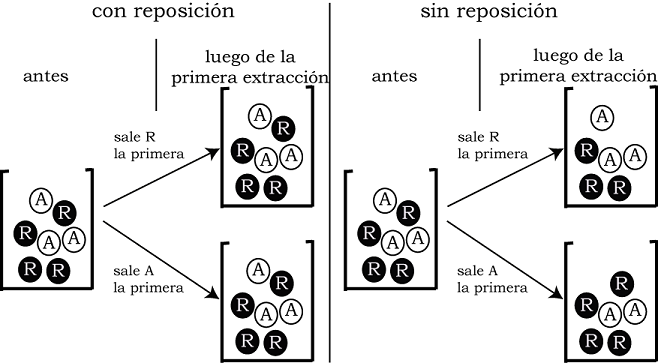
\includegraphics{imagenes/image92} 

}

\caption{Efectos de extraer una ficha sin reponerla o reponiéndola, en las condiciones que quedan para la segunda extracción.}\label{fig:unnamed-chunk-24}
\end{figure}

Este concepto de independencia entre eventos en muy valioso para
analizar uno de nuestros más importantes problemas: las relaciones entre
variables. Veamos su aplicación a la Tabla 2. Si la intención de voto
fuera independiente de la ciudad donde se vive (quiere decir si votaran
del mismo modo personas de las diferentes ciudades) la probabilidad de
encontrar una persona que vote a R si vive en Córdoba sería simplemente
la probabilidad de votar a R, es decir \(P(R/Córdoba)=P(R)\) y del mismo
modo para los demás eventos. En nuestro ejemplo no se obtiene esa
igualdad, ya que:

\(P(R/Córdoba)=300/650=0,46\), mientras que: \(P(R)=600/1530=0,39\)

Por lo que estos eventos no son independientes en sentido estadístico.

Cuando se trataron las relaciones entre variables, se discutió este
problema, al calcular las frecuencias que se esperarían si las variables
fueran independientes. Se concluyó que dos variables son independientes
si la frecuencia relativa de cada celda resulta del producto de las
frecuencias relativas marginales que le corresponden. En el lenguaje de
las probabilidades, encontramos ahora el mismo resultado y lo expresamos
diciendo que si los eventos A y B son independientes, entonces
\[P(A\cap B)=P(A)*P(B)\]

\hypertarget{el-teorema-de-bayes}{%
\subsection{El teorema de Bayes}\label{el-teorema-de-bayes}}

La aplicación que presentamos en este último apartado usa probabilidades
condicionales para deducir la probabilidad que tiene un evento observado
de provenir de diferentes eventos previos. Por esta razón se denomina
también ``teorema de las causas''\footnote{Fue enunciado por Thomas
  Bayes (1702-1761), matemático inglés.}. Nos interesa porque es un
resultado que permite ``aprender de la experiencia'', lo que quiere
decir que da los medios para usar la información disponible para
modificar las probabilidades de determinados eventos. Tiene mucho valor
en Ciencias de la Salud, porque es frecuente conocer cuál es la
probabilidad a priori que un paciente tenga determinada patología (la
prevalencia de la enfermedad) pero, una vez que se dispone de
indicadores clínicos, esa probabilidad cambia. De manera equivalente, si
se conoce cuál es la probabilidad que un alumno termine una carrera
universitaria, esa probabilidad puede modificarse, una vez que se cuenta
con información adicional, como el número de materias que ya ha
aprobado.

De manera general, si \(B_{1}, B_{2}, \ldots, B_{k}\) son eventos
mutuamente excluyentes que completan el espacio muestral (es decir que
la unión de todos esos eventos es \(\Omega\)), y un evento A puede
suceder en intersección con cualquiera de ellos (es decir que A puede
suceder en intersección con \(B_{1}\), o con \(B_{2}\), etc.), lo
esquematizaremos así:

\begin{figure}

{\centering 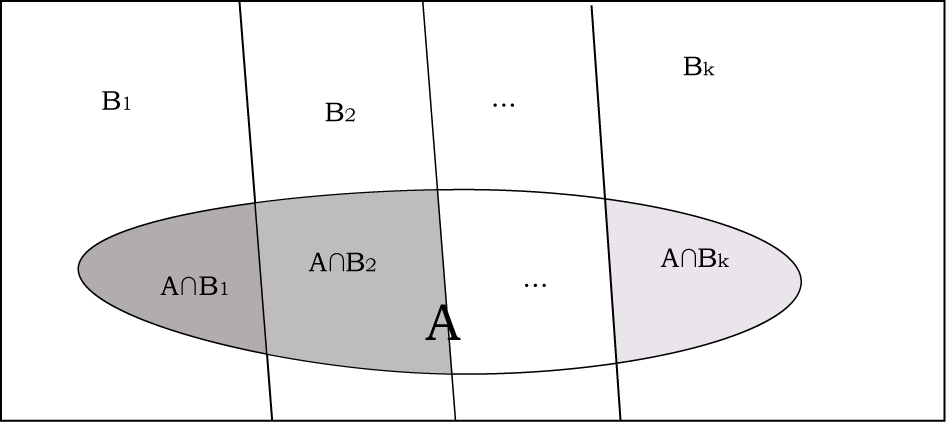
\includegraphics{imagenes/image93} 

}

\end{figure}

Por ejemplo, los eventos \(B\) pueden ser los diferentes tipos de
escuela secundaria de la que provienen los alumnos y el evento \(A\) es
``terminar la carrera''. Hay quienes terminan la carrera (quienes están
dentro de la elipse) y quienes no lo hacen (dentro del rectángulo pero
fuera de la elipse), y tanto unos como otros pueden provenir de escuelas
de cualquiera de los tipos \(B_{1}, B_{2}\) etc. La primera de las
intersecciones (la grisada más oscura) representa a alumnos que cumplen
simultáneamente \(A\) (haber terminado la carrera) y \(B_{1}\) (provenir
de una escuela del tipo que ese grupo define).

Otro ejemplo es que los eventos \(B\) sean solo dos:

\begin{itemize}
\item
  \(B_{1}\): tener una determinada enfermedad
\item
  \(B_{2}\): no tener esa enfermedad
\end{itemize}

\begin{figure}

{\centering 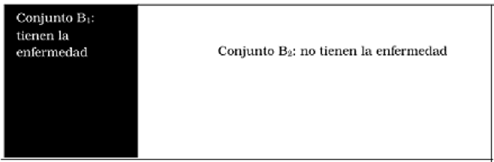
\includegraphics{imagenes/image94} 

}

\end{figure}

Si el evento \(A\) es ``una prueba diagnóstica dio positiva'', aparecen
intersecciones entre el resultado de la prueba y la condición de las
personas a quienes se aplica. La primera es la zona dentro del círculo a
la izquierda: (\(A \cap B_{1}\)), son los casos correctamente
diagnosticados. Los que quedan fuera del círculo a la izquierda
representa casos en los que la prueba no indicó la enfermedad aun cuando
se trataba de personas enfermas, se llaman ``falsos negativos''. A la
derecha, la pequeña parte de círculo es (\(A \cap B_{2}\)) e indica los
casos en que la prueba dio positiva cuando fue aplicada a personas que
no tenían la enfermedad, se llaman ``falsos positivos''. Por último, la
parte blanca del rectángulo a la derecha son los casos en que dio
correctamente negativa en personas que no tenían la enfermedad.

\begin{figure}

{\centering 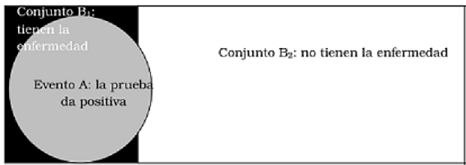
\includegraphics{imagenes/image95} 

}

\end{figure}

Con esta notación y esa relación entre los eventos
\(B_{1}, B_{2}, \ldots, B_{k}\) y \(A\), el teorema de Bayes se expresa
de la siguiente manera:

\[P(B_{j}/A) = \frac{P(B_{j})*P(A/B_{j})}{\sum_{i = 1}^{k}{P(B_{i})*P(A/B_{i})}}\]

El valor de este teorema es que permite pasar de la probabilidad simple
de uno de los eventos \(B\) (en general, del que llamamos \(B_{j}\), a
la probabilidad ``corregida'', a partir de la información que aporta el
evento \(A\). Si se conoce inicialmente la probabilidad del evento
\(B_{j}\), el teorema permite calcular la probabilidad de \(B_{j}\),
luego de haber agregado la condición \(A\).

Veamos un ejemplo sencillo: se dispone de dos frascos, el primero de
ellos tiene 20 fichas azules y 10 rojas, el segundo contiene 20 azules y
20 rojas. Se elige un frasco al azar y luego se extrae de él una ficha,
que resulta ser azul, nos preguntamos por la probabilidad que la ficha
provenga del primer frasco. En ausencia de toda información, los dos
frascos son igualmente probables, por lo que la probabilidad de cada uno
es 0,50: \(P(F1)=0,50\) y \(P(F2)=0,50\). Si la ficha fue extraída del
primer frasco, la probabilidad de que sea azul es:
\(P(A/F1)=20/30=0,67\), mientras que si proviene del segundo frasco es
\(P(A/F2)=20/40=0,50\). La pregunta es por \(P(F1/A)\), debemos invertir
una probabilidad condicional, por lo que usaremos el teorema de Bayes:

\[P(F_{1}/A) = \frac{P(A/F_{1})*P(F_{1})}{P(A/F_{1})*P(F_{1}) + P(A/F_{2})*P(F_{2})}\]

Reemplazando, tenemos:

\[P(F_{1}/A) = \frac{0,67*0,50}{0,67*0,50 + 0,50*0,50} = \frac{0,33}{0,58} = 0,57\]

Este resultado dice que, con el dato que la ficha extraída es azul,
corregimos la probabilidad de provenir del primer frasco, que a priori
era de 0,50; a 0,57. En este sentido la fórmula de Bayes nos permite
usar la información para corregir probabilidades a priori.

En el ejemplo sobre la enfermedad y su diagnóstico, se dispone
inicialmente de la probabilidad que tiene una persona cualquiera de
padecer la enfermedad, esa es \(P(B_{1})\), luego esa probabilidad
cambia cuando se agrega el dato que dice que a la persona la prueba le
dio positiva.

Veamos un ejemplo que presentó Cohen (1994) en un artículo crítico hacia
los procedimientos tradicionales de análisis estadístico. La aplicación
ilustra el aporte del teorema a las interpretaciones de los resultados
que arrojan las pruebas diagnósticas.

La prevalencia de esquizofrenia en adultos es de aproximadamente el 2\%,
que indica que aproximadamente 2 de cada 100 personas en la población
general de adultos padece la enfermedad. Se dispone de un conjunto de
pruebas diagnósticas del que se estima que tiene al menos un 95\% de
precisión al hacer diagnósticos positivos (sensibilidad) y
aproximadamente 97\% de precisión al declarar normalidad
(especificidad).

Para expresar formalmente estos datos, tratamos por un lado, la
situación real, la de ser esquizofrénico o no serlo. Llamamos \(E\) al
evento ``el paciente es esquizofrénico'' y \(noE\) al evento ``el
paciente no es esquizofrénico''. Por lo que, elegida una persona al
azar, y en ausencia de cualquier otra información, su probabilidad de
ser esquizofrénico es \(P(E)=0,02\), la probabilidad que no lo sea es
\(P(noE)=0,98\).

Por otro lado tenemos el resultado del conjunto de pruebas, que pueden
dar positivas o negativas. La sensibilidad se escribe así:
\(P(+/E)=0,95\), que quiere decir que, aplicada a sujetos
esquizofrénicos, el 95\% de las veces la prueba dará un resltado
positivo, que conducirá al diagnóstico correcto de la enfermedad. El
complemento de esa probabilidad, 5\%, es la probabilidad de dar un
resultado negativo ante un caso de alguien que sí es esquizofrénico, se
denomina resultado ``falso negativo'' y solo puede identificarse ante
pruebas posteriores más sensibles o por el desarrollo de otros síntomas,
que dan más elementos para realizar el diagnóstico. Escribimos entonces
que \(P(-/E)=0,05\).

Ante personas que no son esquizofrénicas, la prueba da, en el 97\% de
los casos resultado negativo (correctamente), es decir:
\(P(-/noE)=0,97\). Su complemento, del 3\%, es la probabilidad de hallar
un resultado positivo en alguien que no es esquizofrénico\footnote{Nuevamente
  en este caso, esto puede conocerse a posteriori, luego de otras
  pruebas o del seguimiento del sujeto.}, se denomina ``falso positivo''
y su probabilidad se escribe: \(P(+/noE)=0,03\).

Dado un sujeto cuyas pruebas dan un resultado positivo, nos preguntamos
por la probabilidad que efectivamente sea esquizofrénico. Antes de
conocer la respuesta al problema piénselo un momento por su cuenta y
ofrezca un valor aproximado para esa probabilidad.

Este es un problema que requiere que se invierta una probabilidad
condicional, ya que conocemos la probabilidad de obtener un resultado
positivo si el individuo es esquizofrénico \(P(+/E)\), y queremos saber
la probabilidad que sea esquizofrénico dado que la prueba dio positiva,
que es \(P(E/+)\).

En la aplicación del teorema de Bayes, el universo está compuesto por un
98\% de no esquizofrénicos y un 2\% de esquizofrénicos y la prueba puede
dar positiva tratándose de alguien enfermo (muy frecuentemente) o
estando sano (con poca probabilidad). Reemplazamos en la expresión del
teorema de Bayes y tenemos:

\[P(E/+) = \frac{P(+/E)*P(E)}{P(+/E)*P(E) + P(+/noE)*P(noE)} =\]
\[\frac{0,95*0,02}{0,95*0,02 + 0,03*0,98} = \frac{0,019}{0,019 + 0,029} = 0,396\]

Entonces, si a una persona estas pruebas le han dado resultado positivo,
la probabilidad que efectivamente sea esquizofrénico es menos del 40\%,
que es mucho mayor que la prevalencia en la población general, del 2\%,
pero que no resulta concluyente para el diagnóstico, el cual debe
completarse con otros procedimientos. Es posible que este resultado no
esté cerca de la estimación intuitiva que uno haría y nos pone muy en
alerta sobre la interpretación de pruebas de este tipo. El razonamiento
intuitivo quizás nos habría llevado a creer que alguien a quien la
prueba da positiva tiene muchas posibilidades de tener la enfermedad,
pero no debemos confundir la probabilidad que la prueba de positiva si
se tiene la enfermedad (\(P(+/E)\)) con la probabilidad de tener la
enfermedad si la prueba da positiva (\(P(E/+)\)). Si una persona es
esquizofrénica, la prueba le da positiva en el 95\% de las veces; pero
si da positiva, la probabilidad que sea esquizofrénica es menor al 40\%.

Este resultado no debe conducir a creer que la prueba no sirva para el
diagnóstico. Por el contrario, ante una persona de la que no se tiene
ninguna información, la probabilidad que sea esquizofrénico es 0,02;
cuando se agrega el dato que dice que el test dio positivo, la
probabilidad que sea esquizofrénico asciende a 0,39. Nuevamente, se ve
con claridad cómo este teorema permite usar los resultados de la
experiencia para corregir probabilidades asignadas a priori.

En este ejemplo, la probabilidad de ser esquizofrénico para alguien que
obtuvo resultado positivo en las pruebas es tan baja debido a la baja
frecuencia de la esquizofrenia en la población general (prevalencia),
pero demuestra lo equivocado que puede estarse si no se tienen en cuenta
resultados falso positivo y falso negativo asociados a las pruebas
diagnósticas.

Un abordaje alternativo a este problema es usando una tabla de
contingencia. Suponiendo que aplicamos el conjunto de pruebas a un
universo de un millón de personas y usando las probabilidades enunciadas
antes:

\begin{table}[H]
\centering
\begin{tabular}{lccc}
\toprule
\multicolumn{1}{c}{Condición} & \multicolumn{2}{c}{Resultado de las pruebas} & \multicolumn{1}{c}{Total} \\
\cmidrule(l{3pt}r{3pt}){1-1} \cmidrule(l{3pt}r{3pt}){2-3} \cmidrule(l{3pt}r{3pt}){4-4}
 & Positivo & Negativo & \\
\midrule
\rowcolor{gray!6}  Esquizofrénicos & 19000 & 1000 & 20000\\
No esquizofrénicos & 29400 & 950600 & 980000\\
\rowcolor{gray!6}  Total & 48400 & 951600 & 1000000\\
\bottomrule
\end{tabular}
\end{table}

Queremos responder ¿cuál es la probabilidad que el sujeto sea
esquizofrénico, si sabemos que la prueba le dio positiva? Para ello:

\[P(E/+) = \frac{19.000}{48.400} = 0,39\]

Que es el mismo resultado que obtuvimos aplicando el teorema de Bayes.

La ventaja de la presentación a través de una tabla de doble entrada es
que permite distinguir dos conjuntos de eventos sobre los que tenemos
diferente conocimiento:

\begin{itemize}
\item
  Un \emph{estado de realidad}, que es la condición de esquizofrénico o
  no esquizofrénico del sujeto. Este estado nos es desconocido.
\item
  La \emph{evidencia observable}, que está dada por el resultado de la
  prueba que aplicamos, que conocemos.
\end{itemize}

Como las pruebas no son perfectas, los resultados deben leerse en
términos probabilísticos y no determinísticos.

Cuando ingresemos a inferencia estadística veremos que ésta es la
situación más frecuente: que dispongamos de cierta evidencia y debemos
usarla para tomar una decisión acerca de un estado de realidad al que no
conocemos.

El de Bayes es un teorema de gran importancia, por las consecuencias que
tiene para muchas pruebas diagnósticas que se usan a menudo. Lo que
hemos encontrado también implica el cuidado con que deben leerse los
resultados de pruebas de cualquier tipo: diagnósticos, dosaje de
productos prohibidos en deportistas, pruebas genéticas, etc. Para una
correcta interpretación de los resultados de esas pruebas se deben
conocer cuáles son los errores de tipo ``falso positivo'' y ``falso
negativo'' que las acompañan.

\hypertarget{variables-aleatorias}{%
\subsection{Variables aleatorias}\label{variables-aleatorias}}

Es necesario hacer más explícita una parte del vocabulario que hemos
usado. Al tratar con eventos aleatorios (resultados de experimentos
aleatorios), en algunos hemos usado una notación más textual, como ``que
la moneda salga cara'' y en otros una más numérica, por ejemplo
``\(S=4\)''. De aquí en adelante trabajaremos con la segunda notación
que tiene muchas ventajas. La razón es que pasamos a tratar a los
experimentos como observación de variables, cuyas categorías (o valores)
son los resultados del experimento. En la tirada de la moneda, no es
difícil cuantificar los eventos, podemos elegir cara como lado preferido
y definir la variable X = ``número de caras que se obtienen al lanzar
una moneda equilibrada'', los valores posibles son 0 (si sale cruz) y 1
(si sale cara). En la suma de los puntos de los dos dados, S asume
valores discretos del 2 al 12. La descripción como distribución de
frecuencias que hacíamos antes, se transforma ahora en distribución de
probabilidades y, para los dos ejemplos citados, toma la forma:

\begin{table}[H]
\centering
\begin{tabular}{cc}
\toprule
X = número de caras & \$P(X)\$\\
\midrule
\rowcolor{gray!6}  0 & 1/2\\
1 & 1/2\\
\rowcolor{gray!6}  Total & 1\\
\bottomrule
\end{tabular}
\end{table}

\begin{table}[H]
\centering
\begin{tabular}{cc}
\toprule
S = suma de puntos de dos dados & \$P(S)\$\\
\midrule
\rowcolor{gray!6}  2 & 0.028\\
3 & 0.056\\
\rowcolor{gray!6}  4 & 0.083\\
5 & 0.111\\
\rowcolor{gray!6}  6 & 0.139\\
\addlinespace
7 & 0.167\\
\rowcolor{gray!6}  8 & 0.139\\
9 & 0.111\\
\rowcolor{gray!6}  10 & 0.083\\
11 & 0.056\\
\addlinespace
\rowcolor{gray!6}  12 & 0.028\\
Total & 1.000\\
\bottomrule
\end{tabular}
\end{table}

Estas variables se denominan \textbf{variables aleatorias}, porque sus
valores dependen del azar y serán muy necesarias en todo lo que sigue de
la materia. El aspecto de estas tablas de distribución de probabilidades
es en un todo equivalente al de las de distribución de frecuencias: el
total igual a uno indica la probabilidad del espacio muestral
(\(P(\Omega) = 1\)). Sobre ellas pueden hacerse operaciones similares a
las descripciones de variables ya vistas.

Cuando la variable aleatoria puede asumir valores continuos, ya no es
posible asignar probabilidades individualmente y debe hacerse a través
de intervalos. Es el mismo problema que hallamos en las distribuciones
de frecuencia, y lo resolvemos del mismo modo. Se usan probabilidades
acumuladas, ya sea entre valores de la variable o desde ciertos valores
hacia los mayores o desde ciertos valores hacia los menores\footnote{Sin
  embargo hay algo importante que cambia; porque en lugar de sumar un
  número finito de valores discretos, cuando se trata de variables
  continuas se debe sumar una cantidad infinita de valores
  infinitesimales, ese cambio se refleja en que la operación de suma se
  transforma en otra operación que se llama integral. No disponemos de
  los elementos matemáticos suficientes para ir más allá de esta mención
  imprecisa del concepto, pero tampoco es necesario a los fines de este
  curso.}.

También es posible, sobre distribuciones de probabilidad, calcular
algunas medidas descriptivas, veamos en qué se transforma la media. El
procedimiento para calcularla que hemos visto consiste en multiplicar
cada valor de la variable por su frecuencia y dividir por el total de
casos; para las variables aleatorias eso se hace de una sola vez,
multiplicando cada valor por la probabilidad y se obtiene:

\[E(x) = \sum_{i = 1}^{n}x_{i}*{P(x}_{i})\]

Que se llama \textbf{esperanza matemática}, la indicaremos \(E(x)\).
Aunque esta expresión proviene del cálculo de la media\footnote{Puede
  deducirse esto a partir del cálculo de la media, si se reemplazan las
  frecuencias relativas por las probabilidades de cada valor de la
  variable, tenemos:
  \[\overline{x} = \frac{\sum_{i = 1}^{n}{x_{i}*f_{i}}}{n} = \sum_{i = 1}^{n}x_{i}*\frac{f_{i}}{n} = \sum_{i = 1}^{n}x_{i}*f_{i}^{'} = \sum_{i = 1}^{n}x_{i}*{P(x}_{i}) = E(x)\]},
tiene una diferencia conceptual importante: la media es una medida
resumen, por lo que describe hechos que han sido observados, puede
decirse que hace referencia a algo que ya sucedió. Por el contrario la
esperanza se refiere a eventos que pueden llegar a suceder, por eso
tiene ese nombre, es la expectativa que tenemos sobre el devenir futuro
de un experimento. Uno de los usos más difundidos de este concepto es la
esperanza de vida, que mide el número promedio de años que viviría un
conjunto de personas si a lo largo de toda su vida se mantuvieran las
mismas tasas de mortalidad que en la actualidad (las tasas de mortalidad
se usan para estimar las probabilidades de morir a cada edad). Un
``promedio a futuro'' es una descripción sobre algo que aún no sucedió,
por eso se llama esperanza.

De manera análoga puede calcularse la varianza de una variable
aleatoria, su fórmula es:

\[V(x)=\sum_{i=1}^{n}(x_i-E(x))^{2}*P(x_i)\]

Al referirse a una variable aleatoria, la interpretación de la varianza
difiere levemente de aquella que se usó como medida descriptiva de la
dispersión. Aquí indica el modo en que se alcanzará el valor de la
esperanza. Una varianza grande indica un proceso aleatorio muy variable,
con valores dispares que convergen lentamente al valor de la esperanza.
Por el contrario, un valor pequeño de la varianza indica un proceso más
estable en el que los valores difieren poco de un paso al siguiente y
rápidamente se aproximan a la esperanza.

Un ejemplo común que ilustra el uso de estas medidas es el juego de la
ruleta. En este juego, por cada ficha que se apuesta a un color se
obtiene una de premio si sale ese color y, por cada ficha que se apuesta
a un solo número, se obtienen 35 como premio. En ambos tipos de apuesta,
la ganancia esperada\footnote{Para el caso de ruletas con un solo cero,
  existen algunas que tienen además del cero el doble cero, en esos
  casos la esperanza de pérdida es mayor.} vale -0,027. Esto significa
que, jugando indefinidamente, se espera perder (porque es negativa)
0,027 pesos por cada peso que se apueste; esa es la ganancia esperada
del organizador del juego.

Sin embargo, las varianzas son diferentes; para las apuestas a color,
vale poco menos de 1 y para la apuesta a número único es más de 34. Esto
describe la dinámica del juego; mientras con la primera modalidad se
gana y se pierde a menudo, con la segunda forma de apostar, se pierde
muchas veces y cuando se gana es grande la recompensa. De todos modos en
ambos tipos de apuesta, el balance entre ganancias y pérdidas es
negativo, como lo indica la esperanza.


\end{document}
